\documentclass{article}
\usepackage[utf8]{inputenc}
\usepackage{amssymb,amsmath}
\usepackage[usenames, dvipsnames]{color}
\usepackage{amsthm}
\usepackage{centernot}
\usepackage{mathtools}
\usepackage{ stmaryrd }
\textheight=24cm % высота текста
\textwidth=15cm % ширина текста
\oddsidemargin=1.0cm % отступ от левого края
\topmargin=-1.5cm % отступ от верхнего края
\parindent=24pt % абзацный отступ
\parskip=0pt % интервал между абзацами
\tolerance=2000 % терпимость к "жидким" строкам
\flushbottom % выравнивание высоты страниц
\newtheorem{theorem}{Theorem}
\newtheorem{remark}{Remark}
\newtheorem{proposition}{Proposition}
\newtheorem{definition}{Definition}
\newtheorem{lemma}{Lemma}
\newtheorem{corollary}{Corollary}
\newtheorem{question}{Problem}
\usepackage[russian]{babel}
\usepackage{amsfonts}

\title{Дроби}
\author{~}
\date{~}
\usepackage{natbib}
\usepackage{graphicx}
\graphicspath{{pictures/}}
\DeclareGraphicsExtensions{.pdf,.png,.jpg} 
\begin{document}

\maketitle
\section{Обыкновенные дроби}
До этого мы работали только с натуральными числами. Очень скоро мы познакомимся с другими числами - дробными. Но перед этим нам нужно научиться делать еще одно действие с натуральными числами - деление с остатком. Мы обсуждали ранее, что мы не можем любое натуральное число разделить на любое другое натуральное число: это возможно, только если первое число кратно второму. Тем не менее, мы можем поделить некоторую часть нашего числа на любое другое число. Это называется делением с остатком. Рассмотрим на примере.\\

\textbf{Пример.} Мы хотим разделить число $48$ на $5$. Мы знаем, что $48$ не кратно $5$, но несмотря на это мы можем ответить на вопрос "Сколько раз $5$ помещается в $48$?". Для этого нам нужно найти самое большое число, которое меньше чем $48$ и при этом делится на $5$. Это число $45$. Также мы знаем, что $48$ на $3$ больше, чем $45$. Эту тройку мы и будем называть остатком. Таким образом мы можем записать, что $48 = 5*9 +3$, где $3$ - остаток. Заметьте, что остаток всегда меньше чем делитель (в нашем примере делитель равен $5$).\\

Давайте сформулируем это в общем виде. Для любых натуральных чисел $m, n$ мы можем записать выражение следующего вида: $m = n*a + r$, где $a, r$ - натуральные числа, причем $r < n$.
\subsection{Дробь как результат деления натуральных чисел}
Как бы нам не было комфортно работать с натуральными числами, в жизни возникают ситуации, для которых их не хватает. Например, вы заказали пиццу, она разрезана на 8 частей. Вы съели один кусочек - как математически описать то количество пиццы, которое вы съели? Здесь нам и пригодятся дроби. Запишем это количество как $\frac1{8}$. В этой записи $8$ означает, на сколько кусков мы разделили пиццу, а $1$ - что изначально у нас была только одна пицца. Число такого вида и называется обыкновенной дробью. Число над чертой мы будем называть \textbf{числителем}, а число под чертой - \textbf{знаменателем}.\\

Давайте рассмотрим еще один пример: у нас есть три яблока и мы хотим разделить их на двоих. Сколько яблок получит каждый? Каждый получит по $\frac 3{2}$ яблока, потому что мы $3$ яблока делили на $2$ части.\\

Таким образом мы можем записать результат деления любого натурального числа на любое другое натуральное число: $m : n = \frac m{n}$. В целом, дробь это другой способ записывать деление.
\subsection{Основное свойство дроби}
Представим, что у нас есть торт. Мы разрезали его на 4 части и одну положили себе на тарелку. Таким образом у нас на тарелке лежит $\frac 1{4}$ торта. Если теперь мы каждый кусочек разрежем на три части, всего кусков будет $12$, а у нас на тарелке $3$. Другими словами, у нас на тарелке $\frac 3{12}$ торта. При этом колиество торта не изменилось, а числа стали больше. Это свойство дроби называется основным. Давайте сформулируем его в общем виде.\\

 \newtheorem{Th}{Теорема}
 \begin{Th} \textbf{Основное свойство дроби.}\\
 Если числитель и знаменатель дроби умножить или разделить на одно и то же число, то получится равная ей дробь.
 \end{Th}
Таким образом $\frac1{2} = \frac 2{4} = \frac 3{6} = \frac 4{8} = \frac 5{10} = \dots$

\subsection{Сокращение дробей}
Мы уже знаем, что сы сожем умножить или разделить числитель и знаменатель на одно и то же число. Например, $\frac4{6} = \frac{4:2}{6:2} = \frac2{3}$. Мы будем называть деление числителя и знаменателя дроби на одно и то же число \textbf{сокращением} дроби на это число. В нашем примере мы \textbf{сократили} дробь $\frac4{6}$ на $2$.\\
Любую ли дробь можно сократить? Нет, не любую. Мы уже знаем, что числа могут быть взаимно простыми и не иметь общих делителей. Если числитель и знаменатель дроби взаимно просты, то такую дробь мы не можем сократить, будем называть такие дроби \textbf{несократимыми}.\\
\textbf{Свойство 1.} Если сократить дробь на НОД числителя и знаменателя, то получится несократимая дробь.
\subsection{Сравнение дробей. Приведение к общему знаменателю}
Попробуйте выбрать большую дробь из следующих пар:
\begin{enumerate}
    \item $\frac 1{6}$ и $\frac1{7}$
    \item $\frac5{8}$ и $\frac7{8}$
    \item $\frac {10}{12}$ и $\frac 7{8}$
\end{enumerate}
В первом случае достаточно просто понять, что больше $\frac16$: если мы что-то (тортик, например) разделим на $6$ частей, один кусок будет больше, чем если мы это же что-то разделим на $7$ частей.\\
Во втором случае мы делим на равное количество частей, а значит чем больше изначальное число, тем больше будет результат деления. Соответственно, большее число $\frac78$.\\
В третьям случае все сложнее, ведь у дробей разные и числители, и знаменатели. Но так как мы знаем основное свойство дроби, мы можем \textbf{привести к общему знаменателю} эти дроби. Тогда: \\
$\frac{10}{12} = \frac{10*2}{12*2} = \frac{20}{24}$\\
$\frac78 =\frac{7*3}{8*3} = \frac{21}{20}$\\
Как сравнить дроби с одинаковым знаменателем мы уже знаем: $\frac{20}{24} < \frac{21}{24}$, значит $\frac{10}{12} < \frac78$.

\subsection{Правильная и неправильная дробь}
Во всех примерах, которые были раньше, числитель дроби был меньше чем знаменатель и дроби обозначали какую-то часть от целого (то есть их значение было меньше $1$). Это совершенно не значит, что других ситуаций не может быть.\\

\textbf{Пример.} $1 = \frac11 = \frac22 = \frac33 = \dots$\\
В этом примере числитель и знаменатель дроби равны. Любая дробь, у которой числитель и знаменатель равны, будет равна единице, так как число, деленное на себя, равно единице.\\

Соответственно, если числитель больше, чем знаменатель, дробь больше, чем единица. В этом случае нам интересно сколько единиц "поместится" в это число. В аналогии с тортиками, если нам скажут что у нас есть $\frac{27}{4}$ торта, нам интересно сколько это целых тортов. Самое большое число, которое делится на $4$ и при этом меньше чем $27$, это число $24$. Мы знаем, что $24 = 2*6$, поэтому целых тортов у нас $6$. Если мы "заберем" $~6$ целых тортов, у нас еще останется $\frac34$ торта (потому что $27-24 = 3$). Таким образом у нас есть $6$ целых тортов и еще $\frac34$. Если записатьэто с помощью математического выражения, у нас есть $6 + \frac34$ торта. Мы будем записывать эту сумму так: $6\frac34$. В этом случае $6$ - целая часть числа, а $\frac34$ - дробная. Число, у которого есть и целая, и дробная часть называется \textbf{смешанным числом}.
\newtheorem{Def}{Определение}
\begin{Def}
Дробь называется \textbf{неправильной}, если ее числитель больше знаменателя или равен ему.
\end{Def}

\textbf{Перевод смешанного числа в неправильную дробь.} Мы уже умеем превращать неправильную дробь в смешанное число. Но также мы можем сделать обратное действие: превратить смешанное число в неправильную дробь. Давайте посмотрим как это сделать на том же примере. У нас есть $6\frac34$ торта. Давайте разрежем каждый из шести тортов на $4$ части: получится $6*4 = 24$ кусочка. Еще $3$ куска такого же размера у нас уже было, так что всего у нас $24+3 = 27$ кусков. Таким образом $6\frac34 = \frac{27}4$.\\

Когда мы изучим сложение дробей, мы сможем более строго описать что мы делали в этом примере с тортами. 

\subsection{Сложение и вычетание дробей с одинаковым знаменателем}
Допустим, мы разрезали торт на восемь частей. Сначала вы съели $\frac28$ торта (то есть $2$ куска), а потом еще $\frac18$ (то есть еще один кусок). Сколько всего торта вы съели? Вы съели $2+1=3$ куска, а значит $\frac38$ торта. Таким же образом будет работать и с другими числами.\\
Получается, что чтобы сложить две дроби с одинаковым знаменателем, нужно сложить их числители. Чтобы узнать разность двух дробей с одинаковыми знаменателями, нужно посчитать разность их числителей.\\

Теперь давайте разберемся более строго, как выделить целую часть и перевести смешанное число в неправильную дробь. Запишем наши действия из примеров выше.\\
\textbf{Выделение целой части неправильной дроби.}\\
$\frac{27}4 = \frac{24+3}4 = \frac{24}4 + \frac34 = (24:4) + \frac34 = 6 + \frac34 = 6\frac34$\\
\textbf{Перевод смешанного числа в неправильную дробь.}\\
$6\frac34 = 6 + \frac34$\\
Мы знаем, что $6 = 24:4$, поэтому:\\
$6 + \frac34 = \frac{24}4 + \frac34 = \frac{24+3}4 = \frac{27}4$\\

Давайте научимся складывать и вычитать смешанные числа, при условии, что у их дробных частей равные знаменатели. Конечно, всегда можно перевести дроби обратно в неправильные. С числами, у которых нет целой части, мы уже умеем работать. Давайте научимся работать со смешанными числами, не переводя их в неправильную дробь. Рассмотрим пример.\\

\textbf{Пример 1.} $5\frac49 + 7\frac19 = 5 + \frac49 + 7 + \frac19 = 5 + 7 + \frac49 + \frac19 = 12 + \frac{4+1}9 = 12 + \frac59 = 12\frac59$.\\
Таким образом, чтобы сложить два смешанных числа, нужно отдельно сложить их целые части и дробные части. Чуть сложнее будет, если в результате сложения дробных частей получится неправильная дробь. Рассмотрим еще 2 примера.\\

\textbf{Пример 2.} $5\frac49 + 7\frac59 = 5 + \frac49 + 7 + \frac59 = 5 + 7 + \frac49 + \frac59 = 12 + \frac{4+5}9 = 12 + \frac99 = 12 + (9:9) = 12 + 1 = 13$\\

\textbf{Пример 3.} $5\frac69 + 7\frac59 = 5 + \frac69 + 7 + \frac59 = 5 + 7 + \frac69 + \frac59 = 12 + \frac{6+5}9 = 12 + \frac{11}9 = 12 + \frac{9+2}9 = 12 + \frac99 + \frac29 = 12 + 1 +\frac29 = 13 + \frac29 = 13\frac29.$\\


\subsection{Сложение и вычетание дробей с разными знаменателями}

Мы уже научились складывать и вычетать дроби с одинаковыми знаменателями. Чтобы сложить или вычесть дроби с разными знаменателями, необходимо \textbf{привести их к общему знаменателю}, а далее сложить (вычесть) как дроби с одинаковыми знаменателями.\\

Как привести дроби к общему знаменателю? Для этого нам нужно какое-нибудь число, которое делится на оба наших знаменателя. Самым маленьким таким числом будет НОД знаменателей (нам не обязательно нужно самое маленькое число, но чем меньше числа, тем легче нам с ними работать). Это число и будет новым знаменателем для обеих дробей. Теперь нам нужно каждую дробь привести к общему знаменателю. Мы умеем это делать с помощью основного свойства дроби.\\

\textbf{Пример.} $\frac38 + \frac16 = \frac{3*3}{8*3} + \frac{1*4}{6*4} = \frac9{24} + \frac4{24} = \frac{9+4}{24} = \frac{13}{24}$.\\
С вычетанием все аналогично.

\subsection{Умножение дробей}
Начнем мы с умножения дроби на целое число. Рассмотрим пример.\\
\textbf{Пример.} $\frac27 * 3 = \frac27 + \frac27 + \frac27 = \frac{2+2+2}7 = \frac{2*3}7 = \frac67$.
Обратите внимание, мы умножали дробь на число $3$, в результате числитель умножился на $3$, а знаменатель не изменился. Причем абсолютно аналогично мы можем сделать с любой дробью и любым целым числом. Таким образом, \textbf{чтобы умножить дробь на число, нужно числитель дроби умножить на это число, а знаменатель оставить без изменений.}\\

Теперь научимся делить дробь на число. Рассмотрим несколько примеров.\\
\textbf{Пример 1.} $\frac8{13} : 4 = \frac{8:4}{13} = \frac2{13}$. Мы можем убедиться в том, что мы правильно поделили, умножив результат на $4$. $\frac2{13} * 4 = \frac{2*4}{13} = \frac8{13}$.\\
\textbf{Пример 2.} Хотим узнать значение выражения $\frac67 : 5$. Также как в первом примере мы поступить не можем, потому что числитель дроби не кратен $5$, но мы можем воспользоваться основным свойством дроби и добиться, чтобы числитель делился на $5$.\\
$\frac67 : 5 = \frac{6*5}{7*5} : 5 = \frac{6*5:5}{7*5} = \frac6{7*5} = \frac6{35}$. Мы видим, что в результате деления дроби на число, ее знаменатель умножается на это число, а числитель не меняется.\\

Поскольку мы уже умеем делить и умножать дробь на число, мы можем умножать дробь на дробь. Вы помните, что $m:n = \frac mn$. Воспользуемся этим в следующем примере.\\
\textbf{Пример.} $\frac57 * \frac49 = \frac57 * (4:9) = (\frac57 *4 ) : 9 = \frac{5*4}{7*9}$. \\
Таким образом, чтобы умножить одну дробь на другую, нужно числитель умножить на числитель, а знаменатель на знаменатель.

\subsection{Нахождение дроби от числа}
Представим, что у нас есть $40$ книг. Мы знаем, что из них $\frac38$ - учебники. Сколько у нас учебников?\\
Мы можем решить эту задачу по действиям:\\
1) Найдем $\frac18$ всех книг: $40 * \frac18 = \frac{40}8 = 5$\\
2) Найдем $\frac38$ всех книг: $5 * 3 = 15$\\

Если мы запишем эти два действия в одно выражение, мы получим: $(40 * \frac18) * 3 = 40 * (\frac18 * 3) = 40 * \frac38 = \frac{40*3}8 = 15$.\\
Таким образом, чтобы найти дробь от числа, нужно умножить эту дробь на число.\\
\subsection{Взаимно обратные числа. Деление дробей.}
Если дробь $\frac25$ "перевернуть" (поменять местами числитель и знаменатель), получим дробь $\frac52$. Найдем произведение этих дробей: $\frac25 * \frac52 = \frac{2*5}{5*2} = 1$. 
\begin{Def}
Два числа, произведение которых равно $1$, называют взаимно обратными.
\end{Def}
\textbf{Замечание.} Число $1$ обратно само себе. У числа $0$ нет обратного.

Также мы знаем, что если разделить число само на себя, мы получим $1$. 
Таким образом $\frac25 * \frac52 = 1 = \frac52 : \frac52$. Таким образом, чтобы разделить одну дробь на другую, надо делимое умножить на обратное делителю.\\

\textbf{Пример.} $\frac6{35} : \frac25 = \frac6{35} * \frac52 = \frac37$.

\subsection{Нахождение числа по его части}
Нам известно, что у нас на полке $15$ учебников и это $\frac38$ всех книг, которые у нас есть. Как нам узнать, сколько у нас всего книг? Для этого достаточно ответить на вопрос "какое число нужно умножить на $\frac38$, чтобы получить 15?". Давайте обозначим это число буквой $a$. Тогда:
\begin{align*}
    a*\frac38 &= 15\\
    (a*\frac38) : \frac38 &= 15 : \frac38\\
    a * (\frac38 : \frac38) &= 15 : \frac38\\
    a * 1 &= 15 * \frac83\\
    a &= \frac{15*8}3 = 40\\
\end{align*}
Таким образом, если мы знаем, что $15$ это $\frac38$ всех книг, то всего книг $15 : \frac38$.
\newpage
\section{Понятие десятичной дроби}
В жизни мы часто встречаемся с числами, которые отличаются одно от другого в $10$, $100$, $1000$ и т.д. раз. Поэтому для дробей, знаменатель которых делится на $10$ придумали более простую запись: 
\begin{align*}
 \frac1{10} &= 0,1\\
 \frac1{100} &= 0,01\\
 \frac1{1000} &= 0,001\\
 \frac1{10000} &= 0,0001\\
\end{align*}
И так далее. Эту запись удобно использовать для всех дробей, знаменатель которых кратен десяти.\\
\textbf{Пример}. $\frac8{10} = 0,8;~ \frac{103}{1000} = 0,103;~ 5\frac{27}{100} = 5,27;~ 13\frac3{1000} = 13,003$.\\
Такие дроби мы будем называть \textbf{десятичными}. В десятичной форме записи дробей запятая отделяет целую часть от дробной. Запись дробной части десятичной дроби содержит столько цифр, сколько нулей в записи соответствующей обыкновенной дроби. \\
Когда мы говорили о целых числах, мы также обсуждали их разряды. У дробной части также есть разряды. Например, ниже можно увидеть таблицу разрядов числа $23,70549$.
\begin{figure}[h]
\center{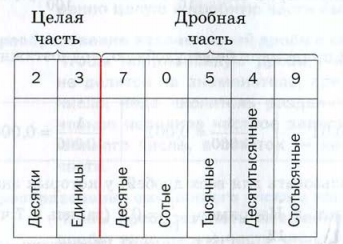
\includegraphics[scale=0.8]{разряды десятичной дроби.png}}
\end{figure}

\textbf{Сравнение десятичных дробей и округление мы обсудим на занятии}.

\section{Сложение и вычитание десятичных дробей}
Сложение и вычитание десятичных дробей происходит аналогично сложению и вычитанию целых чисел: складываем между собой соответственные разряды (единицы с единицами, сотые с сотыми и т.п.).\\
Если мы складываем в столбик, нам нужно чтобы соответсвенные разряды оказались друг под другом. Ровно это произойдет, если мы будем выравнивать числа по запятой: запятая одного числа должна оказаться под запятой другого.\\
Все свойства сложение и вычетания, которые мы уже знаем, сохраняются и для десятичных дробей.

\section{Умножение десятичных дробей}
Об умножении десятичных дробей мы знаем несколько фактов. На занятии мы разберемся, почему это правда, а здесь я напишу только тезисы. Если будет нужно, напишите мне - я скину более подробную информацию.\\

\textbf{Факт 1.} Чтобы умножить десятичную дробь на $10,~ 100,~ 1000$ и т.д., надо перенести в этой дроби занятую вправо соответственно на $1,~2,3$ и и.д. цифры (сколько нулей, столько цифр).\\

\textbf{Факт 2.} Чтобы перемножить две десятичные дроби, надо: 
\begin{enumerate}
    \item Умножить их как натуральные числа, не обращая внимение на запятые;
    \item У произведения оставить после запятй столько цифр, сколько было цифр после запятой у обоих множетелей вместе.
\end{enumerate}
\textbf{Например}, $1,03*2,7 = 2,781$, потому что $103*27 = 2781$.\\

\textbf{Факт 3.} Свойства умножения, которые мы знаем для натуральных чисел, верны и для десятичных дробей.

\section{Деление десятичных дробей}
Все свойства деления для десятичных дробей можно доказать, если перевести десятичные дроби в обыкновенные. Также как в предыдущем пункте, я напишу тезисно результаты, а подробно расскажу на занятии (и скину подробную информацию если понадобится).\\

\textbf{Факт 1}. Чтобы разделить дробь на $10,~ 100,~ 1000$ надо в этой доби перенести запятую влево на $1,~2,~3$ и т.д. цифры соответственно.\\

\textbf{Факт 2}. Если делимое и делитель увеличить одновременно во сколько-то раз, то частное не изменится. Это следует из основного свойства дроби (числитель и знаменатель можно домножить на одно и то же число). В частности, мы можем увеличить делимое и делитель увеличить в $10,~100,~1000$ и т.д. раз.\\
\textbf{Например}, $24,8 : 0,04 = 248 : 0,4 = 2480 : 4 = 620$.\\

\textbf{Факт 3}. Чтобы разделить десятичную дробь на десятичную дробь, нужно увеличить делимое и делитель в некоторое количество раз, чтобы делитель стал натуральным числом, а потом десятичную дробь разделить на натуральное число.\\

Скорее всего, это звучит не понятно, так что раздерем на примере. Заодно поймем, как делить десятичную дробь на натуральное число в столбик.\\
Мы хотим разделить $4,352$ на $1,7$. Воспользуемся фактом 2: $4,352:1,7 = 43,52 : 17$. Теперь поделим в столбик. Сначала мы будем делить также, как делили натуральные числа, но когда дойдем до запятой, поставим запятую в частном. И продолжим делить как натуральные числа. 
\begin{figure}[h]
\center{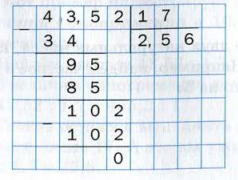
\includegraphics[scale=0.6]{Деление в столбик.PNG}}
\end{figure}
\end{document}
